\documentclass[a4paper,12pt]{ujarticle}
\usepackage{listings,jlisting}
\usepackage[top=30truemm,bottom=30truemm,left=25truemm,right=25truemm]{geometry}
\usepackage[dvips]{graphicx}
\usepackage{siunitx}
\begin{document}
\title{マイクロコンピュータ 後期期末レポート}
\author{電気情報工学科2年 \\ E1533 西総一朗}
\date{2017年2月10日提出}
\maketitle
\begin{itemize}
 \item 光が流れるプログラム(片道バージョン)
 \item 光が流れるプログラム(往復バージョン)
\end{itemize}
\clearpage
\tableofcontents
\clearpage
 \section{リスト5-5(光が流れるプログラム(片道バージョン))}
  \subsection{プログラム概要}
  8個あるLEDの1個を右端や左端から順次点灯することによって、光が流れるように見えるプログラム。
  \subsection{ソースコード}
   \begin{lstinputlisting}[basicstyle=\ttfamily\footnotesize, frame=single]
   {../5-5/5-5.asm}
   \end{lstinputlisting}
  \subsection{フローチャート}
  \begin{figure}[htbp]
   \begin{center}
     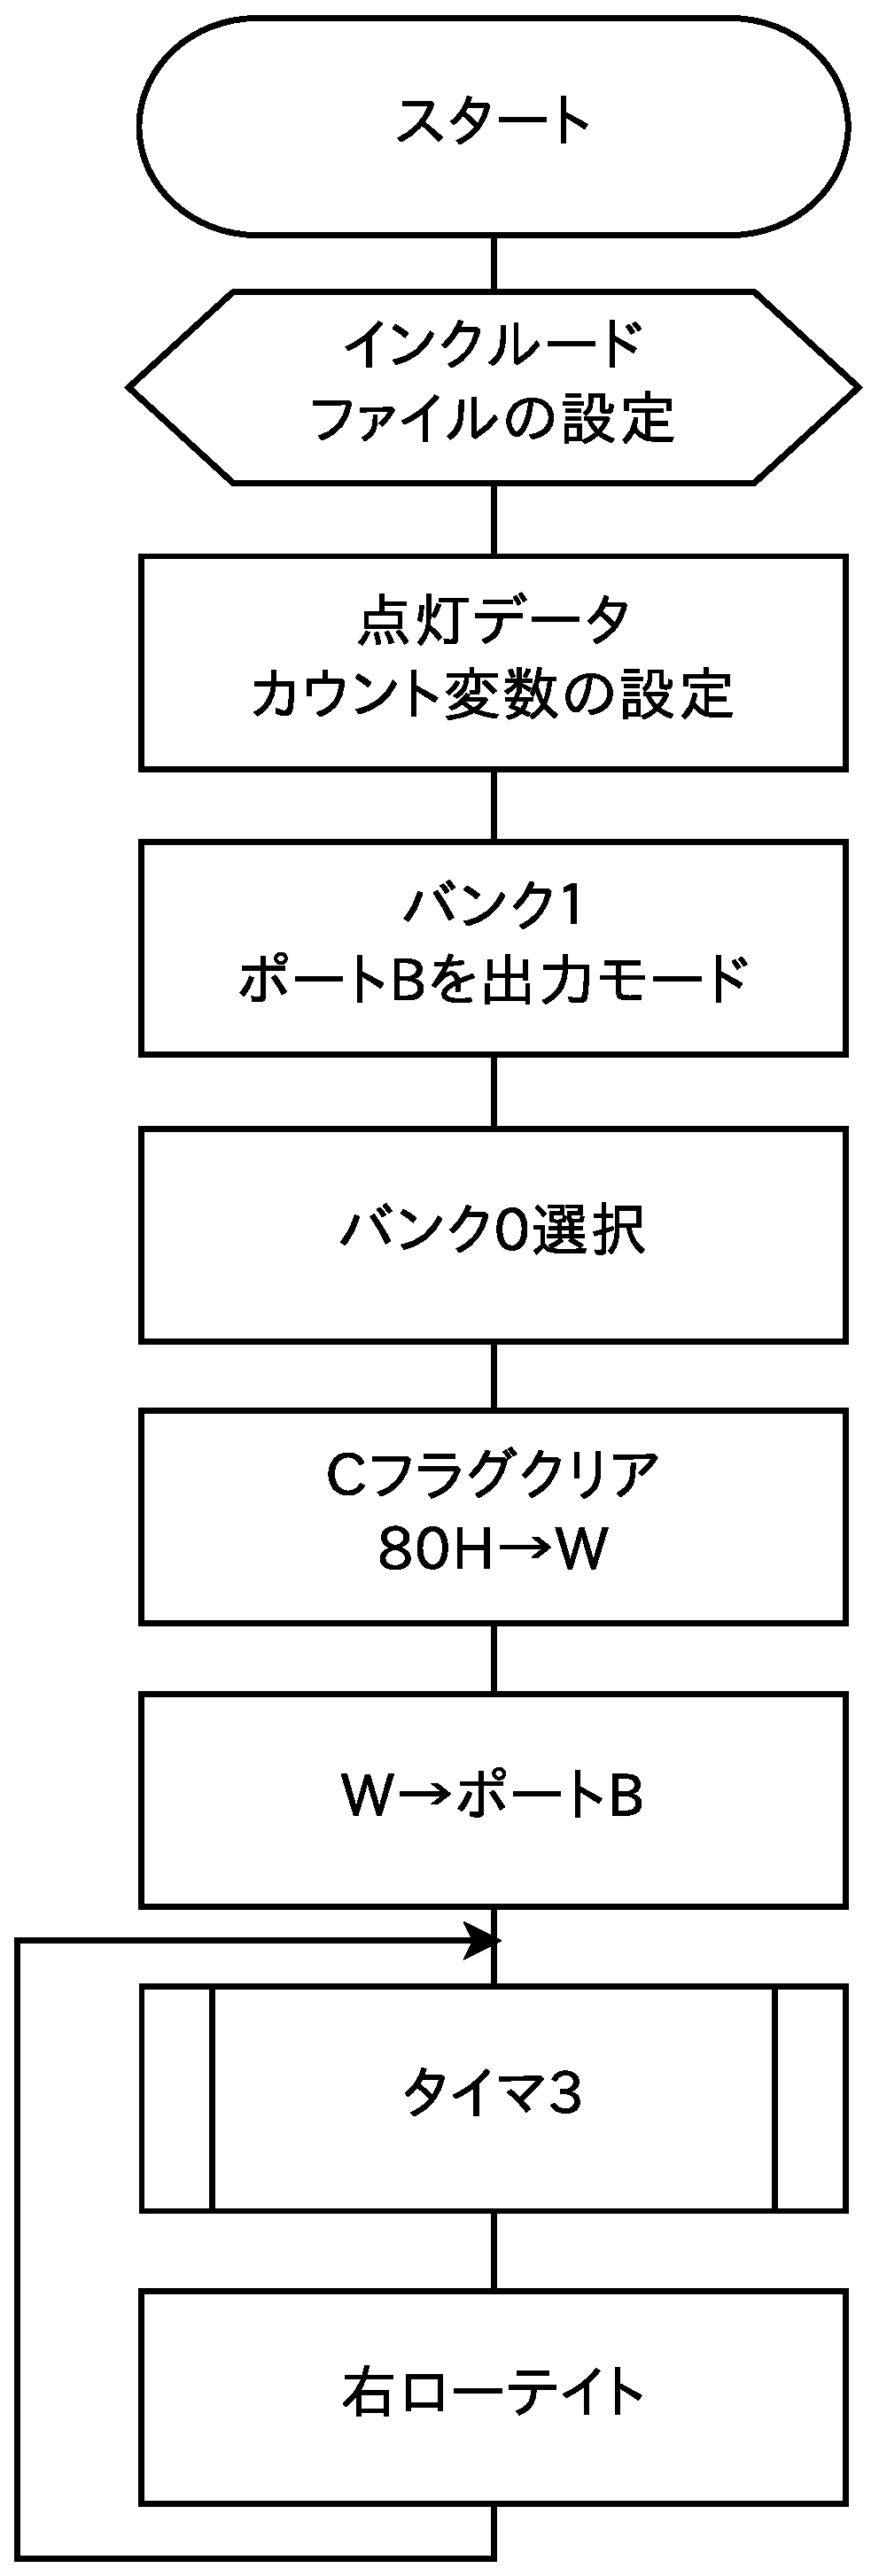
\includegraphics[height=145mm]{Diagram5-5.eps}
   \end{center}
   \caption{フローチャート}
   \label{fig}
  \end{figure}
  \clearpage
  \subsection{実行結果}
  \begin{eqnarray*}
   {80}_{16} = 10000000_2 \\
   ●○○○○○○○ \\
   {40}_{16} = 01000000_2 \\
   ○●○○○○○○ \\
   {20}_{16} = 00100000_2 \\
   ○○●○○○○○ \\
   {10}_{16} = 00010000_2 \\
   ○○○●○○○○ \\
   {8}_{16}  = 00001000_2 \\
   ○○○○●○○○ \\
   {4}_{16}  = 00000100_2 \\
   ○○○○○●○○ \\
   {2}_{16}  = 00000010_2 \\
   ○○○○○○●○ \\
   {1}_{16}  = 00000001_2 \\
   ○○○○○○○● \\
   ●:点灯○:消灯
  \end{eqnarray*}
  このように、0.5秒毎に光る場所が、右に動いていく。右端に到達すると、すべてのLEDが消えるタイミングがある。
  \subsection{考察}
  ローテイト(RRF)命令は1ビットずつ右にシフトさせるもので、16進数において1ビット右にシフトさせることは2で割ることになる。
  RRF命令はCフラグを経由してデータを回転するので端に到達したら一時的に全部が消える瞬間がある。
  この操作を0.5秒のタイマルーチンで呼び出すことで、0.5秒毎に光が動いているように見える。\\

  PICのクロック周波数は$10\si{\mega\hertz}$なので、1クロックあたりは
    \[
     \frac{1}{10\si{\mega\hertz}} = \SI{0.1}{\mu\second}
    \]
    4クロックで1サイクルなので、1サイクルあたりは
    \[
     \SI{0.1}{\mu\second} \times 4 = \SI{0.4}{\mu\second}
    \]
     \begin{figure}[htbp]
      \begin{center}
       \includegraphics[width=130mm]{Diagram5.eps}
      \end{center}
      \caption{サイクル数}
      \label{fig:sicle}
     \end{figure}
     TIMER1のサイクル数は図\ref{fig:sicle}より、249サイクルだとわかり、
     \[
      \SI{0.4}{\mu\second} \times 249 = \SI{99.6}{\mu\second} \approx \SI{0.1}{\milli\second}
     \]
     TIMER1では$\SI{0.1}{\milli\second}$消費される。\\
     このTIMER1をTIMER2では100回、TIMER2では50回呼び出しているので、
     \[
      \SI{0.1}{\milli\second} \times 100 \times 50 = \SI{50}{\milli\second} = \SI{0.5}{\second}
     \]
     合計で$\SI{0.5}{\second}$のタイマールーチンである。
  \subsection{練習問題5.6}
     \subsubsection{問題}
     リスト5-5を点灯が左方向に移動するように変更せよ。
     \subsubsection{回答}
  \begin{lstlisting}[basicstyle=\ttfamily\footnotesize, frame=single]
;       RRF     PORTB,1     ;右方向
        RLF     PORTB,1     ;左方向
  \end{lstlisting}
  このようにRRFをRLFに変更する。
  16進数で1ビット左にシフトさせることは2をかけることになる。
  \subsection{練習問題5.7}
  \begin{lstlisting}[basicstyle=\ttfamily\footnotesize, frame=single]
TIMER1  MOVLW   D'62'       ;0.1ms
        MOVWF   CNT1
LOOP1   NOP
        DECFSZ  CNT1,F
        GOTO    LOOP1
        RETURN

TIMER2  MOVLW   D'100'      ;10ms
        MOVLW   CNT2
LOOP2   NOP
        CALL    TIMER1
        DECFSZ  CNT2,F
        GOTO    LOOP2
        RETURN

TIMER3  MOVLW   D'10'       ;0.1s
        MOVWF   CNT3
LOOP3   NOP
        CALL    TIMER2
        DECFSZ  CNT3,F
        GOTO    LOOP3
        RETURN
  \end{lstlisting}
  このようにタイマのところを変更する。
  \clearpage
 \section{リスト5-6(光が流れるプログラム(往復バージョン))}
  \subsection{フローチャート}
  \begin{figure}[htbp]
   \begin{center}
    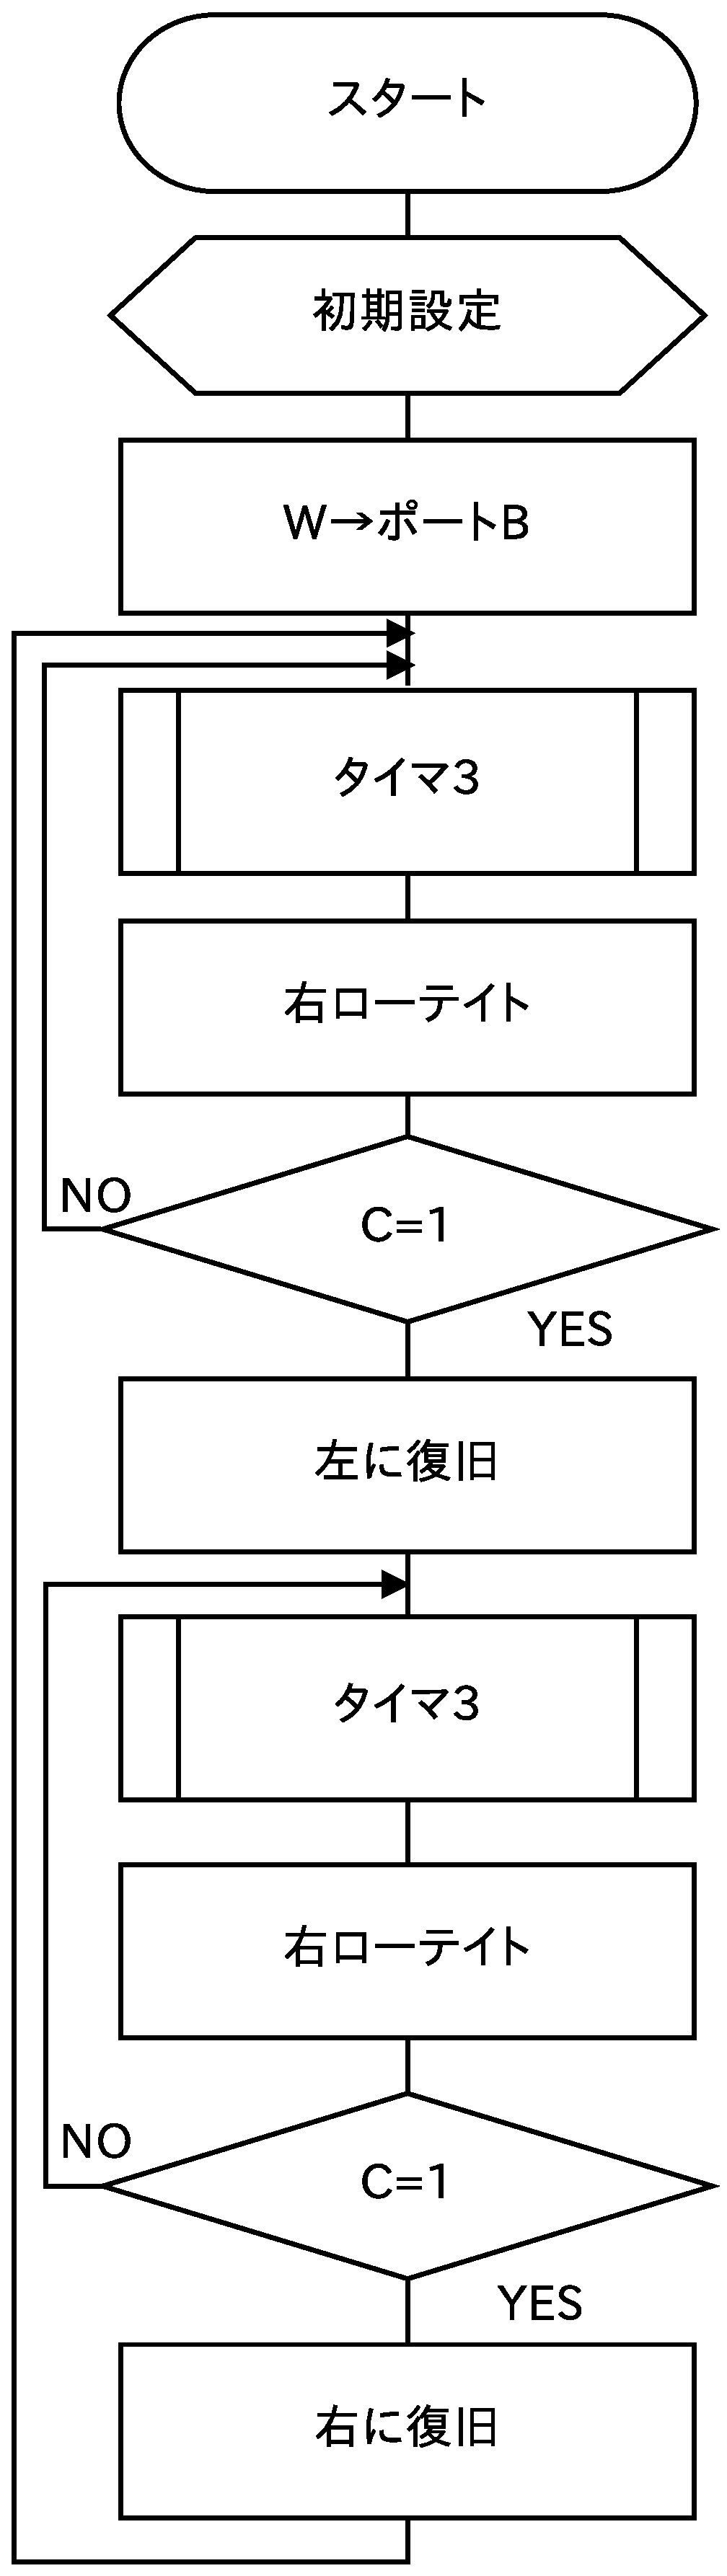
\includegraphics[height=145mm]{Diagram5-6.eps}
   \end{center}
   \caption{フローチャート}
   \label{fig}
  \end{figure}
  \subsection{ソースコード}
  \begin{lstinputlisting}[basicstyle=\ttfamily\footnotesize, frame=single]
   {../5-6/5-6.asm}
  \end{lstinputlisting}
  \subsection{実行結果}
  \begin{eqnarray*}
   {80}_{16} = 10000000_2 \\
   ●○○○○○○○ \\
   {40}_{16} = 01000000_2 \\
   ○●○○○○○○ \\
   {20}_{16} = 00100000_2 \\
   ○○●○○○○○ \\
   {10}_{16} = 00010000_2 \\
   ○○○●○○○○ \\
   {8}_{16}  = 00001000_2 \\
   ○○○○●○○○ \\
   {4}_{16}  = 00000100_2 \\
   ○○○○○●○○ \\
   {2}_{16}  = 00000010_2 \\
   ○○○○○○●○ \\
   {1}_{16}  = 00000001_2 \\
   ○○○○○○○● \\
   {2}_{16}  = 00000010_2 \\
   ○○○○○○●○ \\
   {4}_{16}  = 00000100_2 \\
   ○○○○○●○○ \\
   {8}_{16}  = 00001000_2 \\
   ○○○○●○○○ \\
   {10}_{16} = 00010000_2 \\
   ○○○●○○○○ \\
   {20}_{16} = 00100000_2 \\
   ○○●○○○○○ \\
   {40}_{16} = 01000000_2 \\
   ○●○○○○○○ \\
   {80}_{16} = 10000000_2 \\
   ●○○○○○○○ \\
   ●:点灯○:消灯
  \end{eqnarray*}
  0.2秒毎に光るところが右に動いていき右端になったら、左方向に戻ってくる。
  \subsection{考察}
  ローテイト命令は、Cフラグを含めてシフトするので、光が右端(0ビット目)または左端(7ビット目)に移動したことをCフラグで判定。
  Cフラグが1の場合はオーバーフローかアンダーフローしているので、過分ローテイトの復旧(2ビット復旧)することで、なめらかに移動するように見える。
  \subsection{練習問題5.8}
  \begin{lstlisting}[basicstyle=\ttfamily\footnotesize, frame=single]
LEDD     EQU     80H    ;左端から右方向にスタート
;LEDD    EQU     01H    ;右端から左方向にスタート
  \end{lstlisting}
  このように、LEDDのデータを80Hから01Hに変更する。
  \subsection{練習問題5.9}
  過分ローテイトの復旧がないと、すべてのLEDが点灯しない瞬間が生じる。
  \subsection{練習問題5.10}
  \clearpage
\end{document}